\chapter{All-sky Analysis}
  \label{sec:analysis}

    What we present here is a test of the generalizability of results from Ch. \ref{ch:lori}, which focused on a particular structure on the sky, $\lambda$~Orionis.
    We first would like to note that ``all-sky analysis'' can be a bit misleading. The term tends to lead readers to the idea of a definitive study, answering a particular question for any given position on the sky.  While a truly all-sky analysis would be ideal, signal-to-noise constraints (mainly at high galactic latitudes), as well as confusion along the line of sight (mainly in the galactic plane), make a uniformly powerful study of the whole sky very challenging. Here we will indeed show results for the entire sky as a benchmark analysis, but for the core analysis we must mask certain regions dominated by systematic effects in order minimize biases for particular wavelenghts.



\section{Pixel masking and resolution}
    \subsubsection{Smoothing}
        As in Ch. \ref{ch:lori}, this approach applies to a spatial resolution of approximately ~1$^{\circ}$. The resolution limimtation is imposed by the PC microwave component maps, which list an `effective resolution' of 60arcminutes \citep{planck15X}. Thus we must apply a smoothing to most of our input datasets, which have native resolutions of a much finer scale (see Tab. \ref{tab:data}), and Fig. \ref{fig:AME_contours}. The data also come in a wide range of beam shapes with their own degrees of uncertainty, thus we conservatively smooth all of the data in the same way, using a circular Gaussian beam, to have ~1$^{\circ}$ FWHM resolution. we ar We start with an all-sky AME to IR comparison, looking for global patterns among all pixels (except those within 10$^{\circ}$ of the ecliptic plane.)

    \subsection{Pixel mask}
      \paragraph{Zodical light}
        To keep our analysis comparable to previous works, we exclude pixels within 10$^{\circ}$ of the ecliptic plane. Even though we use the Zodi-subtracted maps (\citep{kelsall98, kondo16}), the Zodi residuals are still problematic (especially in the MIR.) Espeically at high ecliptic latitudes, the relative uncertainty of the Zodi-level is not well estimated; S/N may significantly reduced in for faint pixels, mainly for the 9 through 25~$\mu$m.

     \paragraph{Point Sources}
       The Planck Collaboration provides masks of the pixels they find to include point sources. In our analysis, we mask pixels which are flagged as being point-source contaminated, in the most heavily affected maps: Planck/HFI 857 GHz and Planck/LFI 30 GHz.


  \subsection{All-sky cross correlations}

        \begin{figure}

          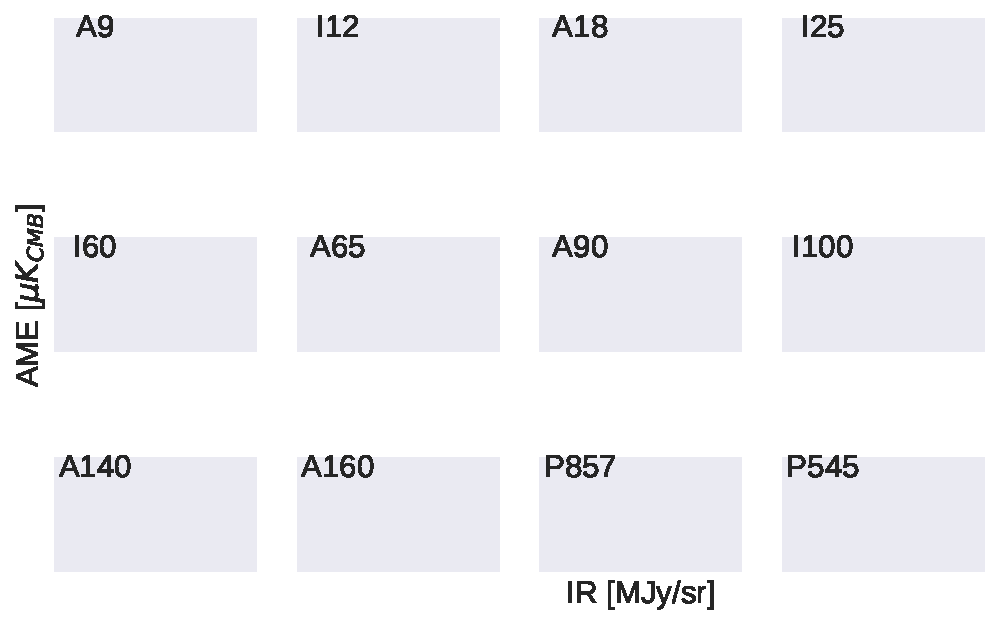
\includegraphics[width=\textwidth]{../Plots/AMEvsDust_allsky_allbands.pdf}
          \centering
          \caption{ALL-SKY kernel density estimates of 12-band infrared photometry against the PR2 AME map. Pixels within 10$^{\circ}$ of the ecliptic plane are excluded. 'A' indicates AKARI; 'D', DIRBE; 'I', IRAS, and 'P' Planck. The number after each letter indicates the band central nominal wavelength in microns (or frequency in GHz, in the case of the Planck bands.) }
          \label{fig:AMEvsDust_allsky_allbands}
        \end{figure}

        \begin{figure}
          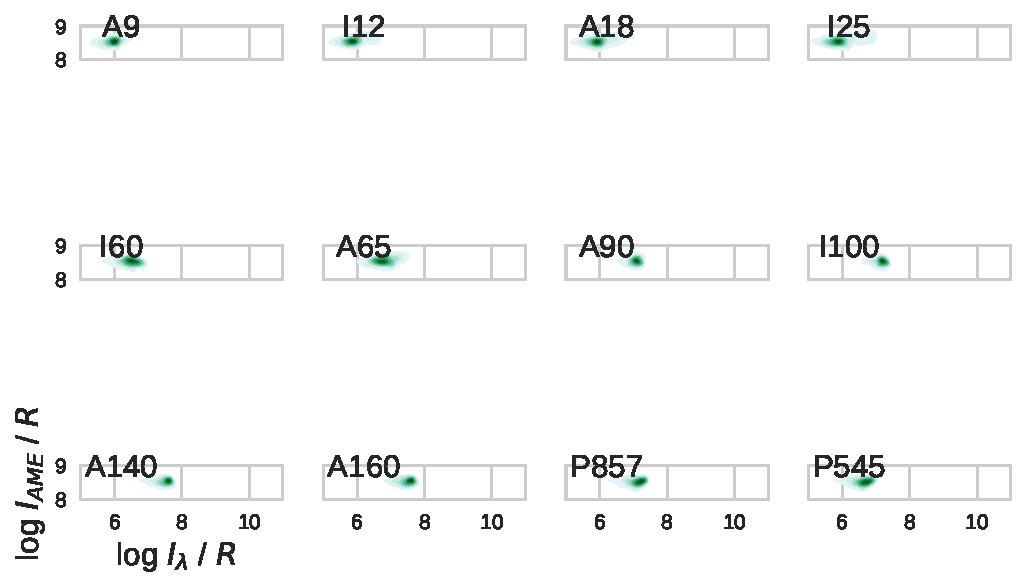
\includegraphics[width=\textwidth]{../Plots/AMEvsDust_allsky_allbands__mpsub_Rnorm_kde.pdf}
          \centering
          \caption{Similar comparison to Fig. \ref{fig:AMEvsDust_allsky_allbands}, with both the IR and the AME intensities scaled by the PR2 dust radiance ($R$) for each pixel. }
          \label{fig:AMEtoRvsDusttoR_allsky_allbands}
        \end{figure}


    \subsubsection{Unmasked Comparison}
        In order to look more closely how the the AME to IR relationship varies with wavelength, we first do a simple cross-correlation test. Figure \ref{fig:AMEvsDust_allsky_allbands} show the Spearman's $\rho$ ($r_{S}$) corrlation matrix for the unmasked sky.
        \begin{figure}
          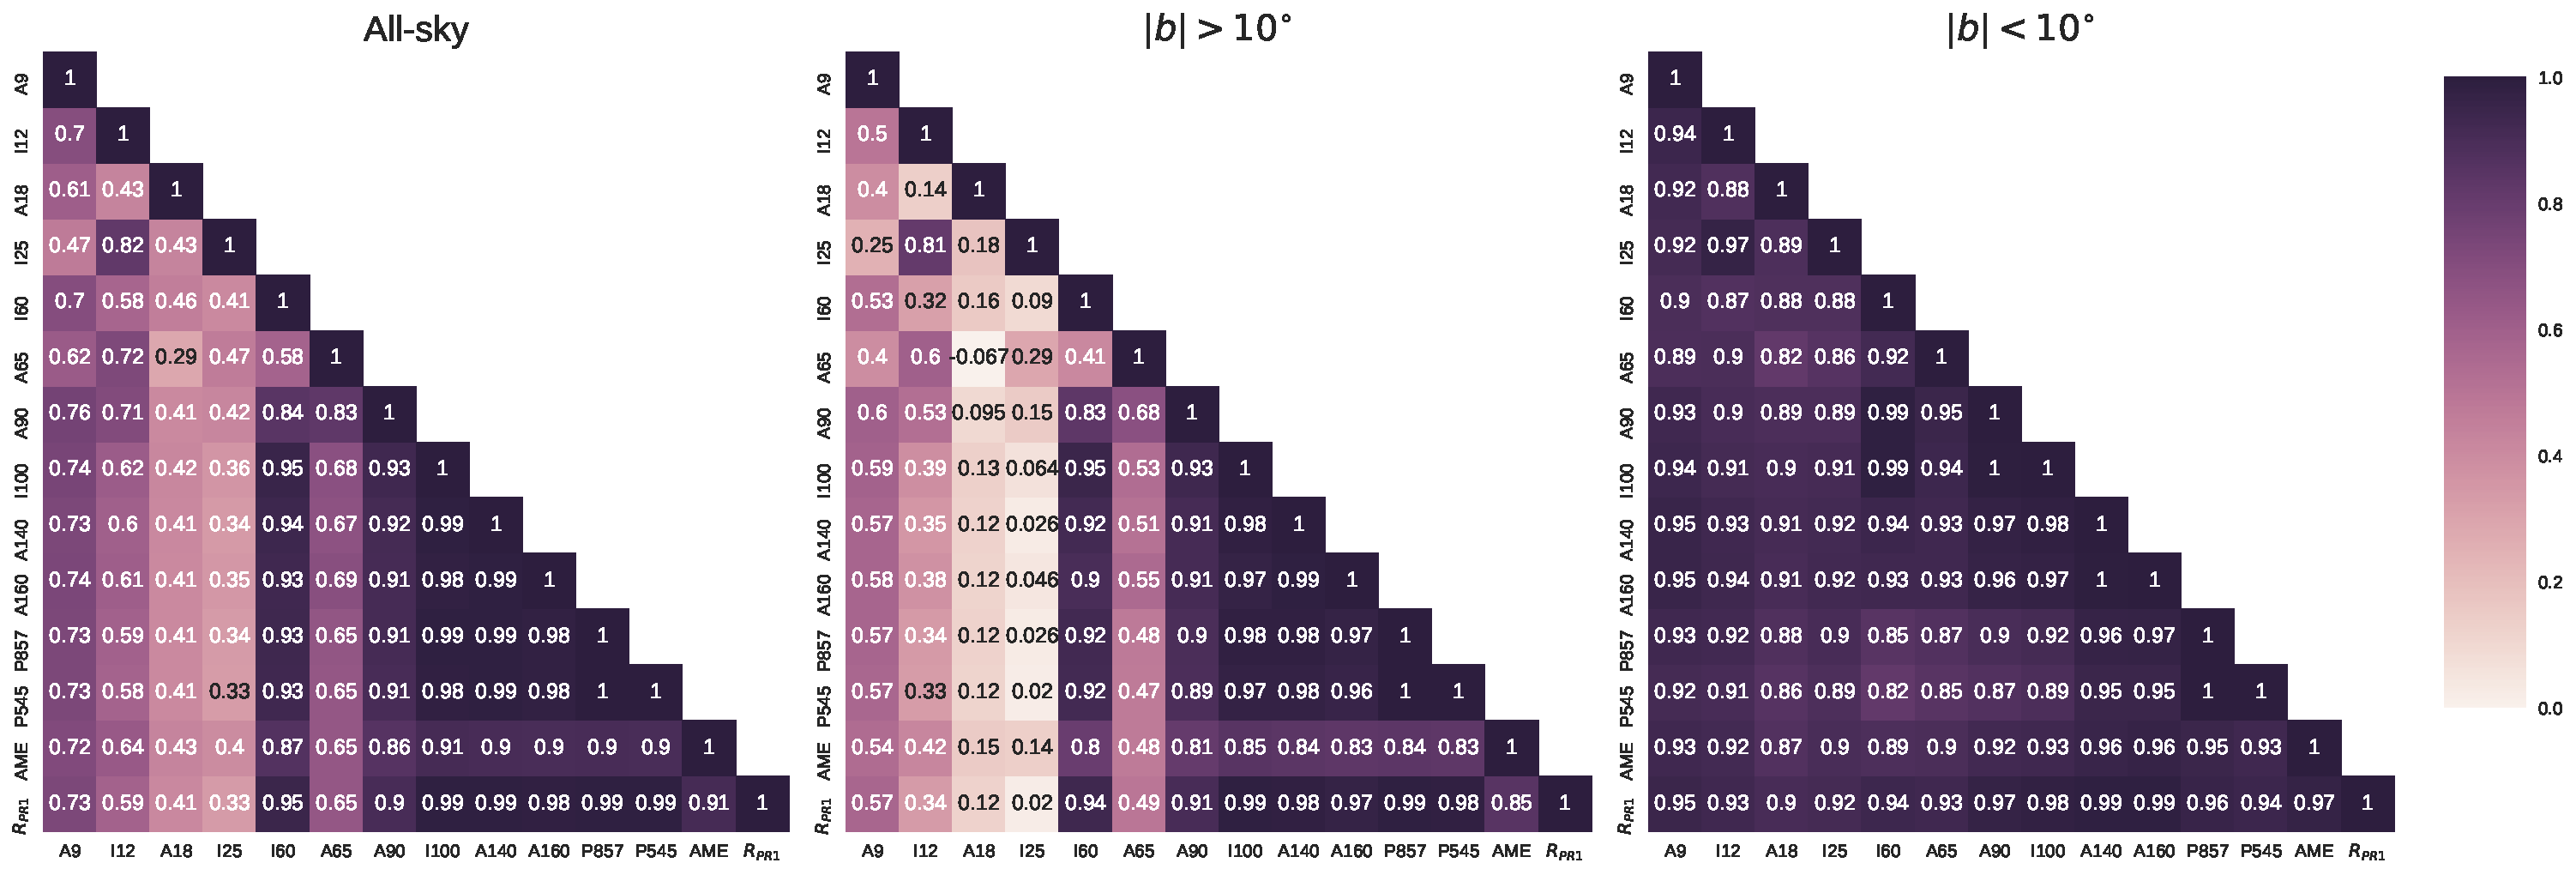
\includegraphics[width=\textwidth]{../Plots/all_bands_corr_matrix_wAME_spearman.pdf}
          \centering
          \caption{ALL-SKY cross-correlation matrix for the 12 infrared bands sampled, and the AME map. THe color-scale indicates ($r_{S}$). Results are based on the full sky (excluding pixels within 10$^{\circ}$ of the ecliptic plane).}
          \label{fig:AME_IR_crosscorr_allbandsg}
        \end{figure}
        Unmasked that is, except for the Zodical light mask. This comparison however may largely be affected by differences is resiudual Zodical light, even in regions far from the ecliptic plane. Galactic plane confusion also plays a role- note how all of the mapss essentially agree with one another at latitudes lower than 15 degrees. Differing noise of the maps, derived mainly from the different sensitivities of the instruments themselves, as well as varying scanning strategies and data processing pipelines, leads to a divergence of the maps with one another at higher galactic latitudes. As well as the IR bands from \ref{tab:data}, we also show the correlations with various ancilliary maps, as well as the PC microwave component maps. The two AME components are shown separately.

    \subsubsection{Masked Comparison}
        We define a pixel mask somewhat similar to that used by \cite{hensley16}, in that we adopt the Planck point source masks, and exclude pixels near the galactic plane and near the ecliptic plane. We do not use the WISE data however, thus our S/N threshold is based on the AKARI 9 micron map rather than WISE 12 micron. Finding that such a S/N threshold eliminates the vast majority of pixels beyond 30 degrees galactic latitude, with the pronounced exception of regions affected by stray moonlight, we choose simply to mask all pixels beyond 30 degrees latitude. We find this to be the simplest, most easily reproducable mask which minimizes S/N biases, point source contamination, and solar system systematic effects in our combined dataset. The AKARI 9 micron masked-sky map is shown in figure \ref{fig:A9_masked_map}. The intensity correlation-matrix for such a masked comparison is shown in \ref{fig:all_bands_corr_matrix_wAME_spearmanintensity_maskall}, with the correlation method and maps considered exactly the same as for the unmasked comparison and Fig. \ref{fig:AMEvsDust_allsky_allbands}.
        \begin{figure}
          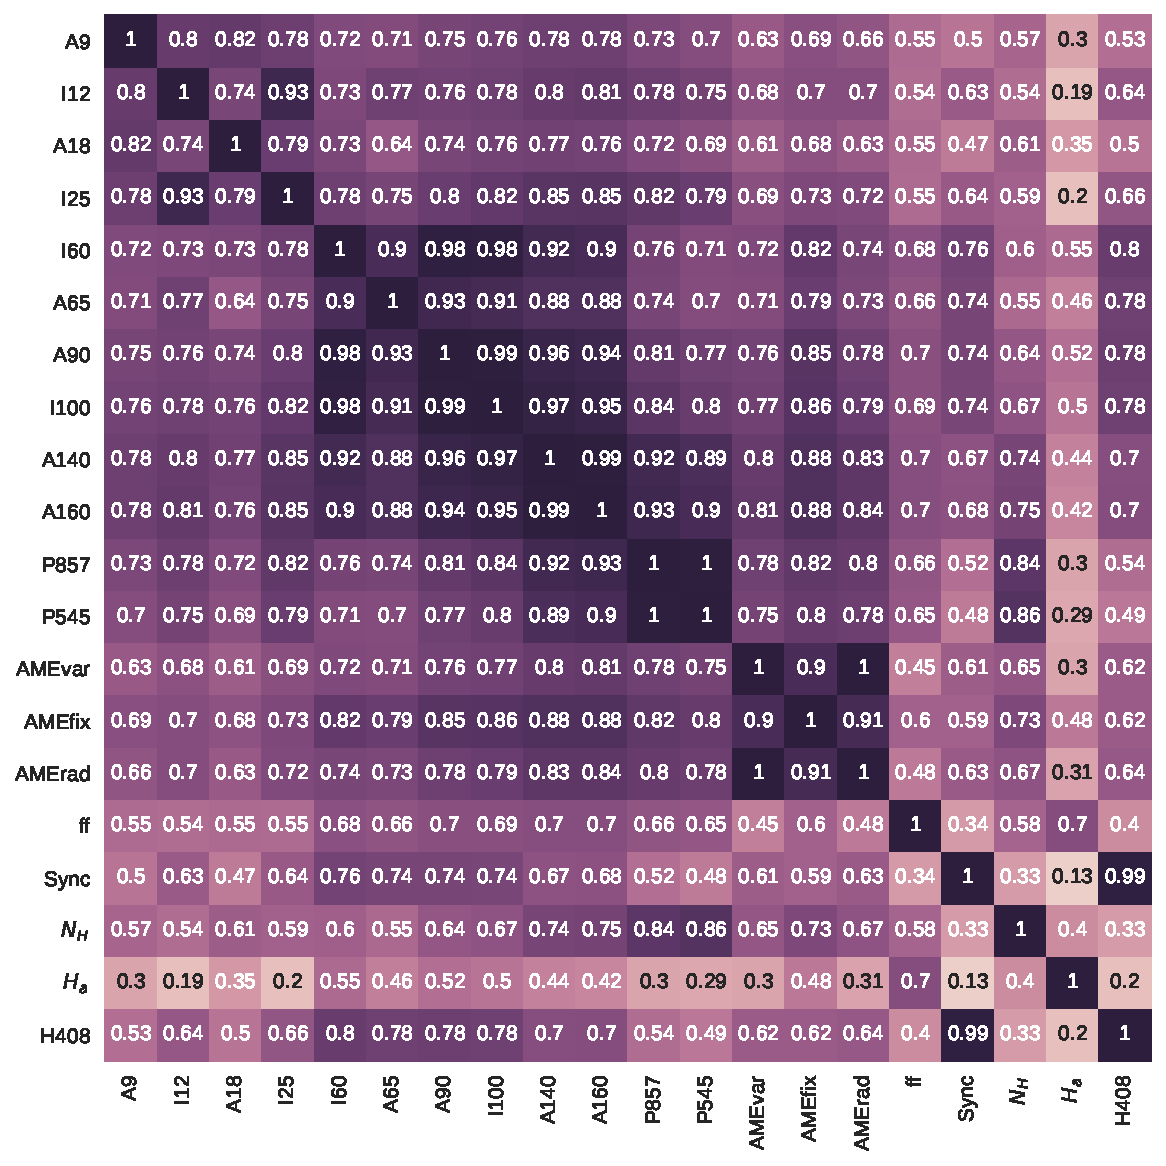
\includegraphics[width=\textwidth]{../Plots/ch_allsky/all_bands_corr_matrix_wAME_spearmanintensity_maskall.pdf}
          \centering
          \caption{.}
          \label{fig:all_bands_corr_matrix_wAME_spearmanintensity_maskall}
        \end{figure}

        \paragraph{Bootstrap test}
            In addition, for the masked comparison, we carry out a boostrap analysis similar to that discussed in Ch \ref{ch:lori} and Fig. \ref{fig:bootstrap_vs_AME}. The Spearman rank correlation coefficents $r_{S}$ of all of the bands, in intensity, vs. the $AME{var}$ component are shown. This is done only for the masked case, due to the computational challeneges presented by a well-sampled bootstrap of all ~700,000 pixels in the full sky. Because the mask applied here leaves us with approximately 1/7 of the sky, a bootstrap of N iterations with N pixels becomes tractable (though ideally we would prefer $n_{iterations} > n_{samples}$). We show the comparison only for the $AME_{var}$ component also due to computational constraints. The $r_{s}$ distributions for each IR band vs. AME are shown in Fig. \ref{fig:bootstrap_vs_AME_allsky_masked}
            \begin{figure}
                 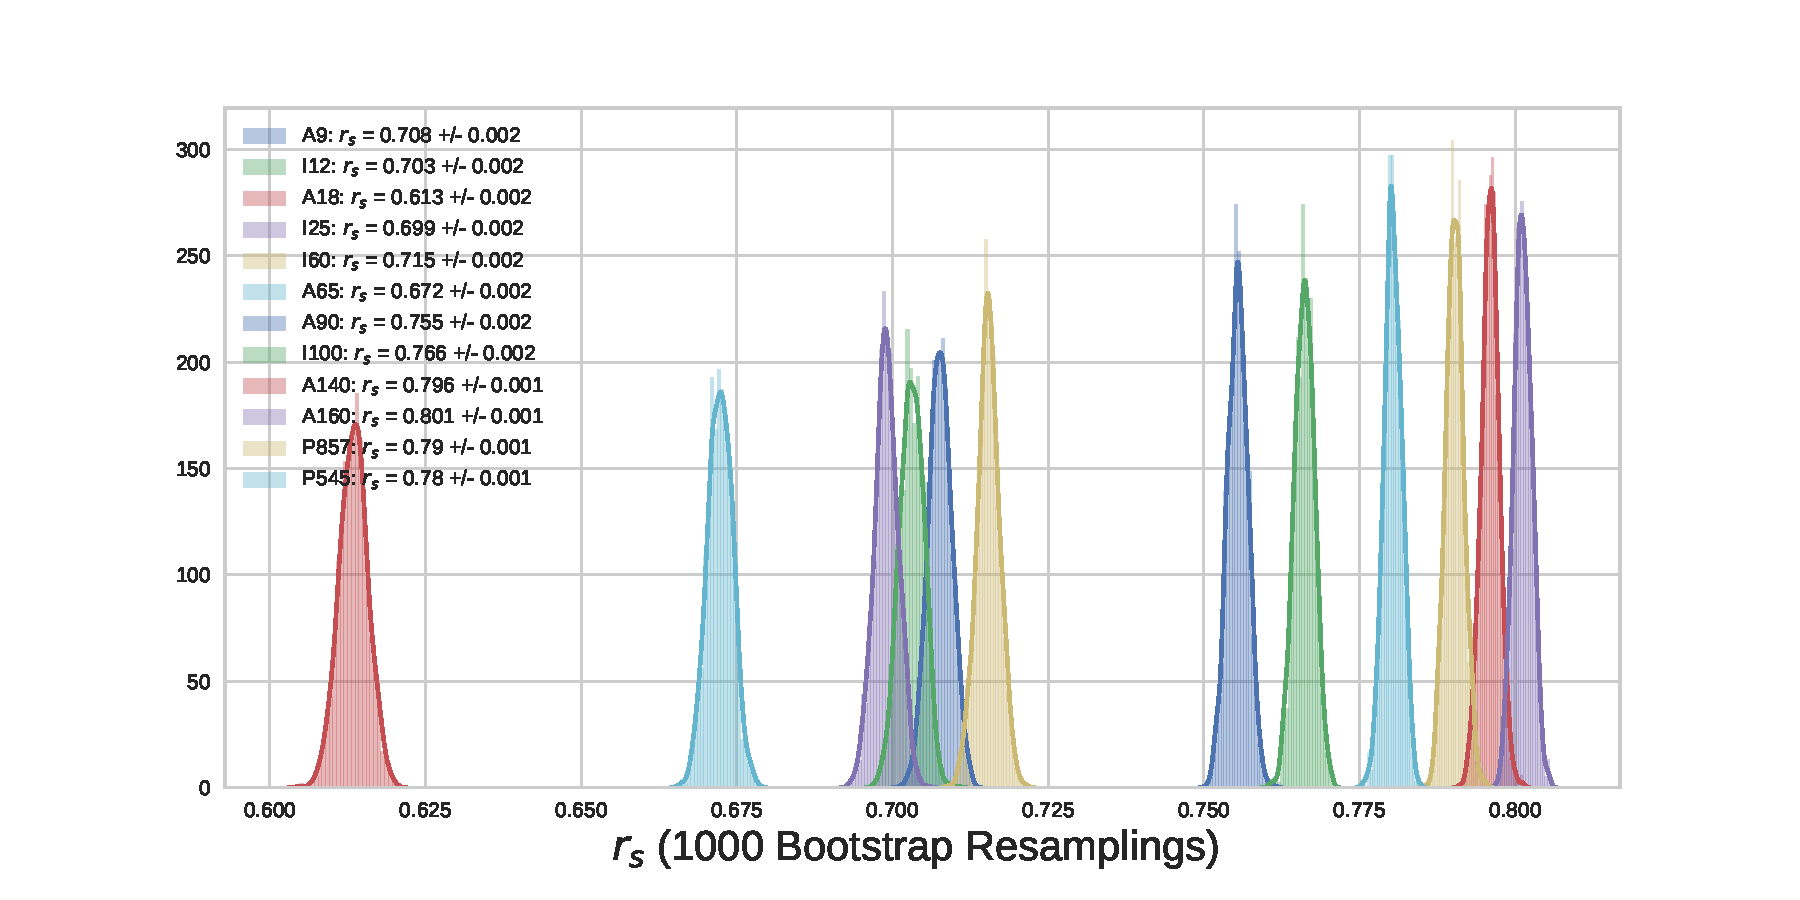
\includegraphics[width=\textwidth]{../Plots/ch_allsky/bootstrap_vs_AME_spearman_maskall_i1000.pdf}
                 \centering
                 \caption{.}
                 \label{fig:bootstrap_vs_AME_allsky_masked}
            \end{figure}

       \begin{figure}
         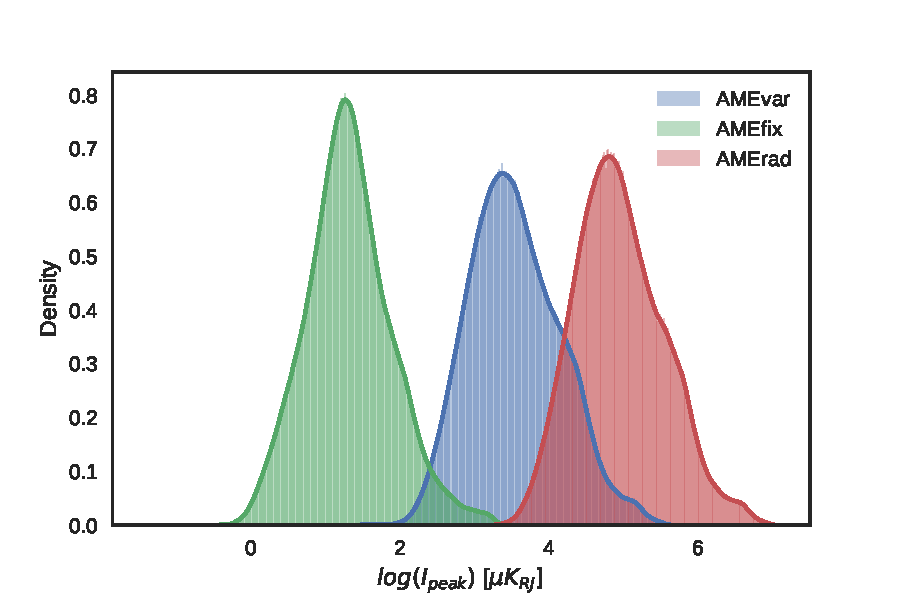
\includegraphics[width=\textwidth]{../Plots/ch_allsky/AME_comps_distplot.pdf}
         \centering
         \caption{Histograms of the peak intensity AME maps calculated from the original COMMANDER-AME reference frequency maps. AMEvar (blue) indicates the distribution of all pixels in the map, with intensities calculated at their peak frequencies (see Fig.} \ref{fig:AME_commander_freqdist}). AMEfix gives the peak intensity of the spatially-constant frequency component.
         \label{fig:AME_comps_distplot}
       \end{figure}

       \begin{figure}
         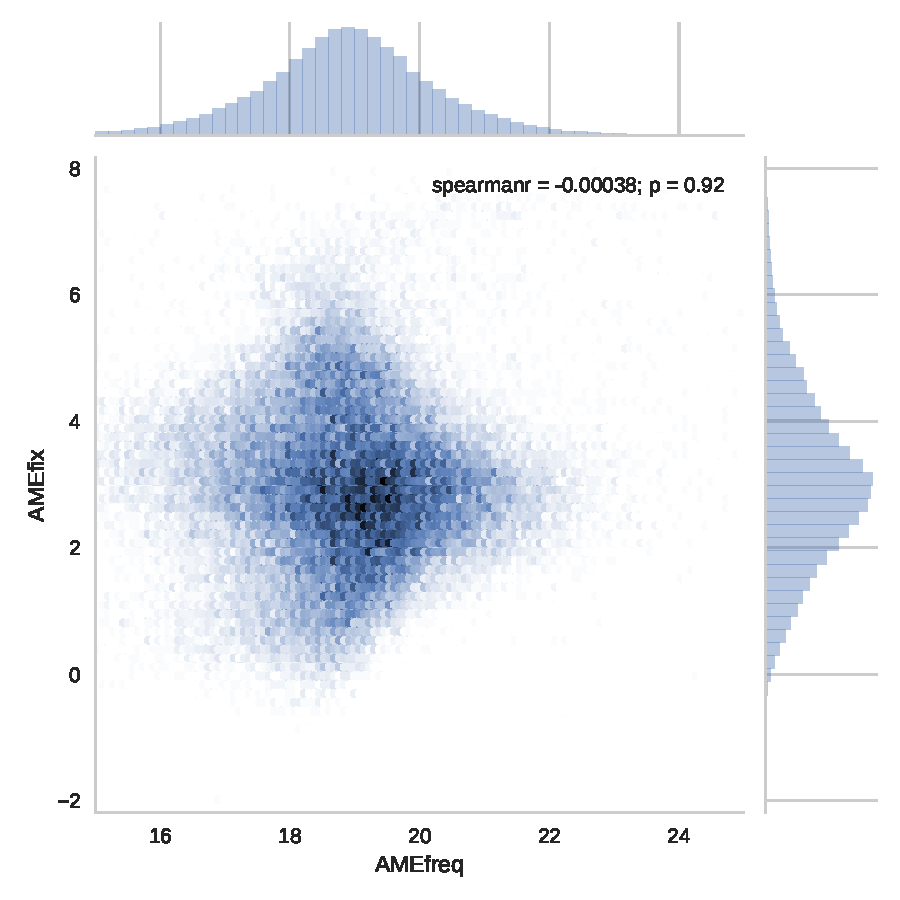
\includegraphics[width=\textwidth/3]{../Plots/ch_allsky/AMEfreq_vs_fix.pdf}
         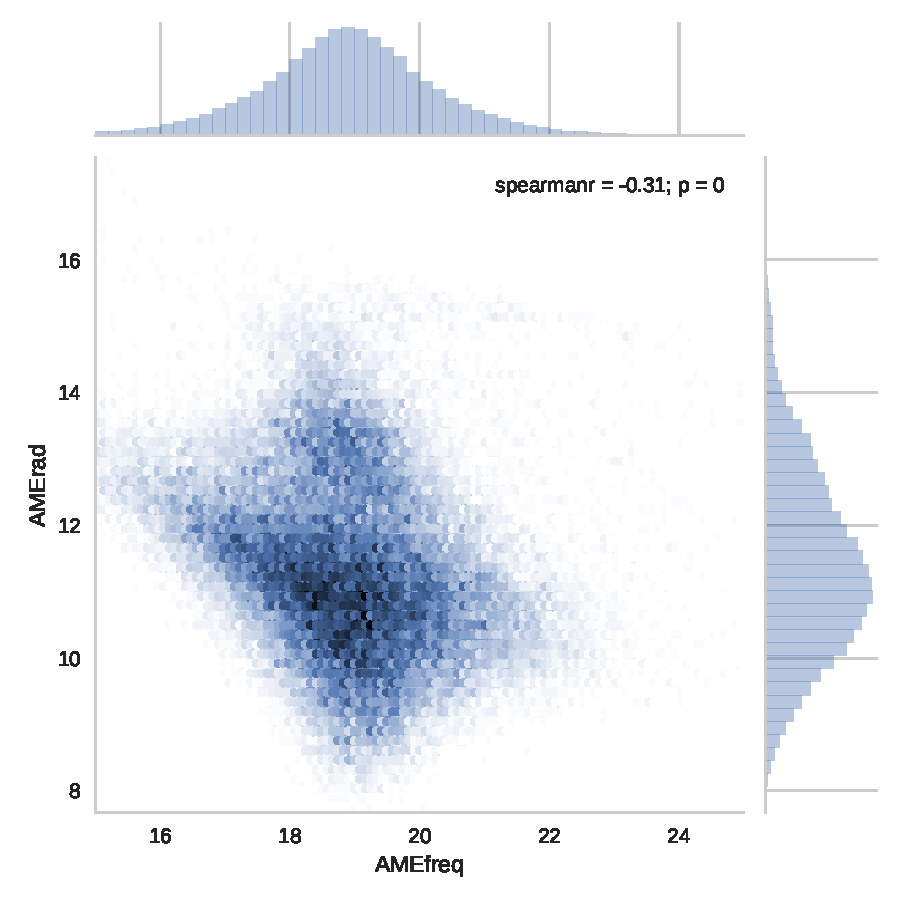
\includegraphics[width=\textwidth/3]{../Plots/ch_allsky/AMEfreq_vs_rad.pdf}
         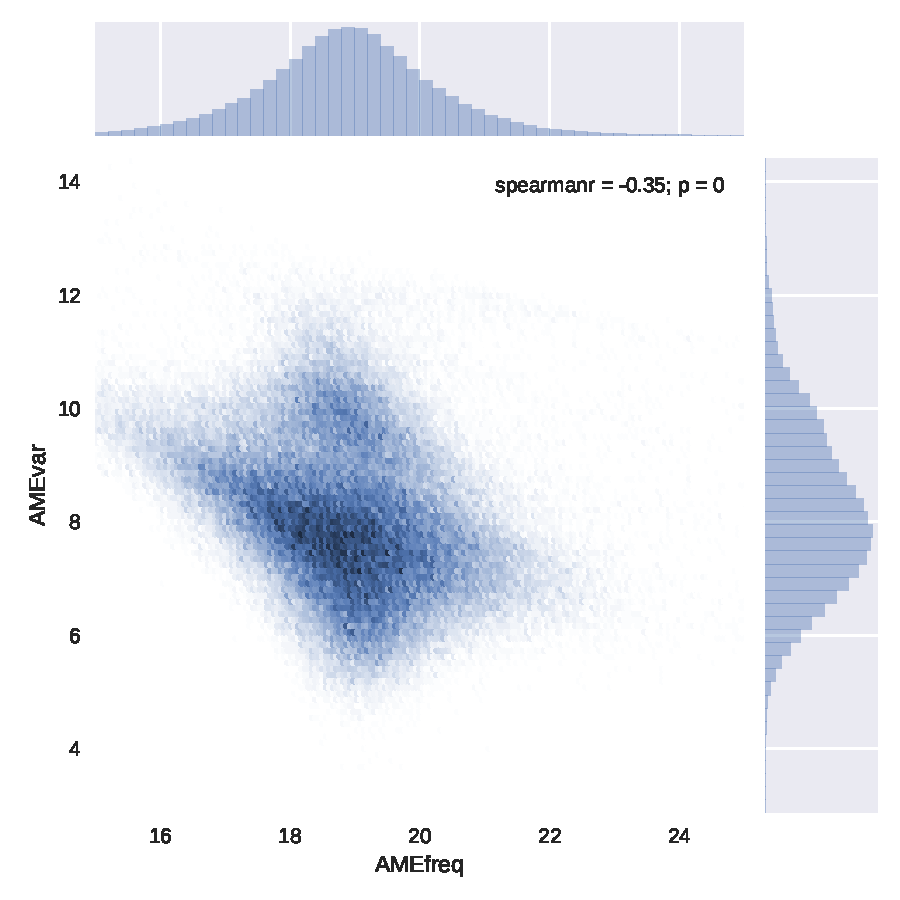
\includegraphics[width=\textwidth/3]{../Plots/ch_allsky/AMEfreq_vs_var.pdf}
         \centering
         \caption{AME intensities vs. peak frequencies..}
         \label{fig:AMEfreq_vs_int}
       \end{figure}

     Figure \ref{fig:AME_IR_crosscorr_allbandsg} visualizes the cross-correlation matrix for each of the IR bands. The AME does not show a strong correlation with other bands at $|l|>10$. At $|l|<10$, the FIR bands show stronger correlation. The PAH-tracing bands show a stronger correlation than bands at 18 to 60~$\mu$m, but weaker than AME vs. the FIR bands.

  \section{Spatial variaton of correlations}
    To understand how these trends may vary across the sky, we produce an all-sky maps of $r_{s}$ for AME vs. IR emission. From the NSIDE~256 input maps of AME and 4 IR wavelength maps, we produce NSIDE~8 maps of $r_{s}$. These maps are shown in Fig. \ref{fig:Spearman_Map_nside8_AMEtoIR}.




      \begin{figure}
        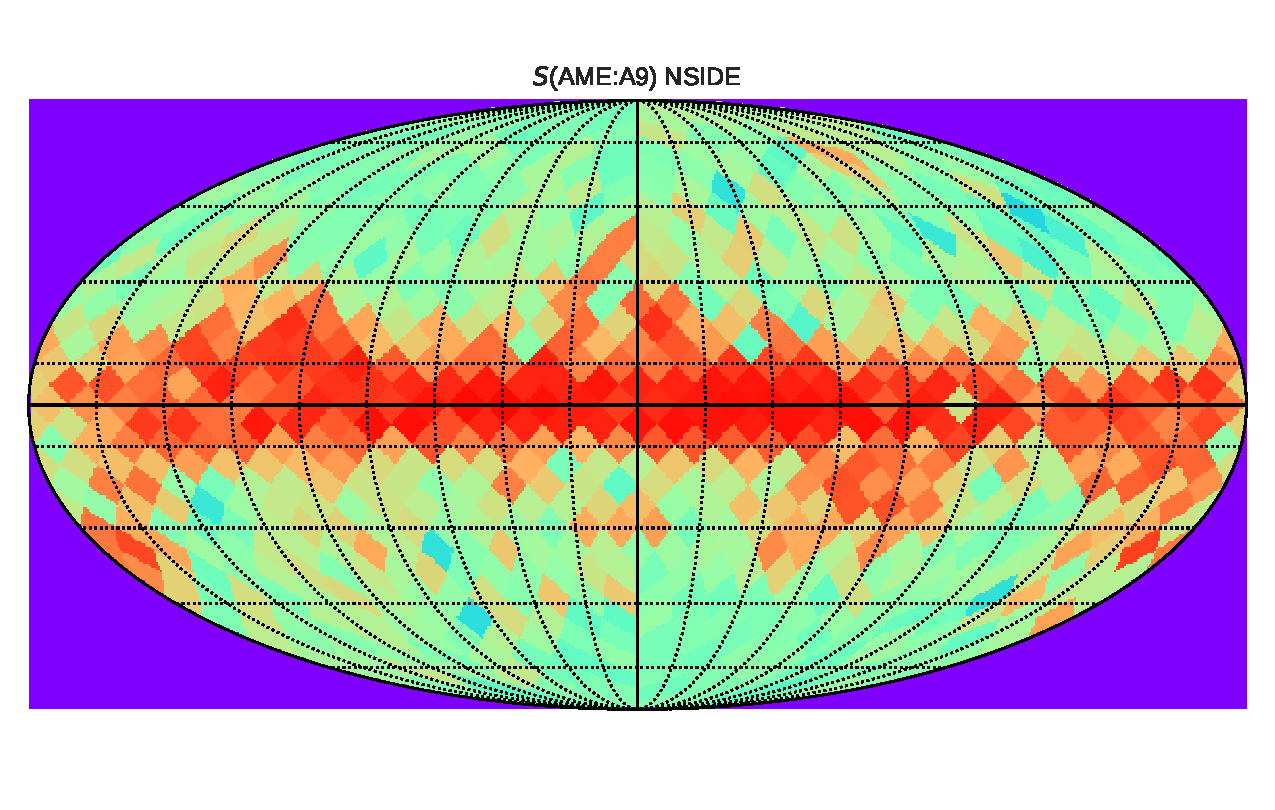
\includegraphics[width=\textwidth]{../Plots/Allsky_Corr/Spearman_Map_nside8_AMEtoA9.pdf}
        \centering
        \caption{Spatial map of $r_{s}$ between the AME and IR intensity for 4 bands:$9~\mu{}m$, $12~\mu{}m$, $25~\mu{}m$, and $140~\mu{}m$. $r_{s}$ is calculated for all NSIDE~256 pixels within each NSIDE~8 pixel-sized bin.}
        \label{fig:Spearman_Map_nside8_AMEtoIR}
      \end{figure}

      \begin{figure}

        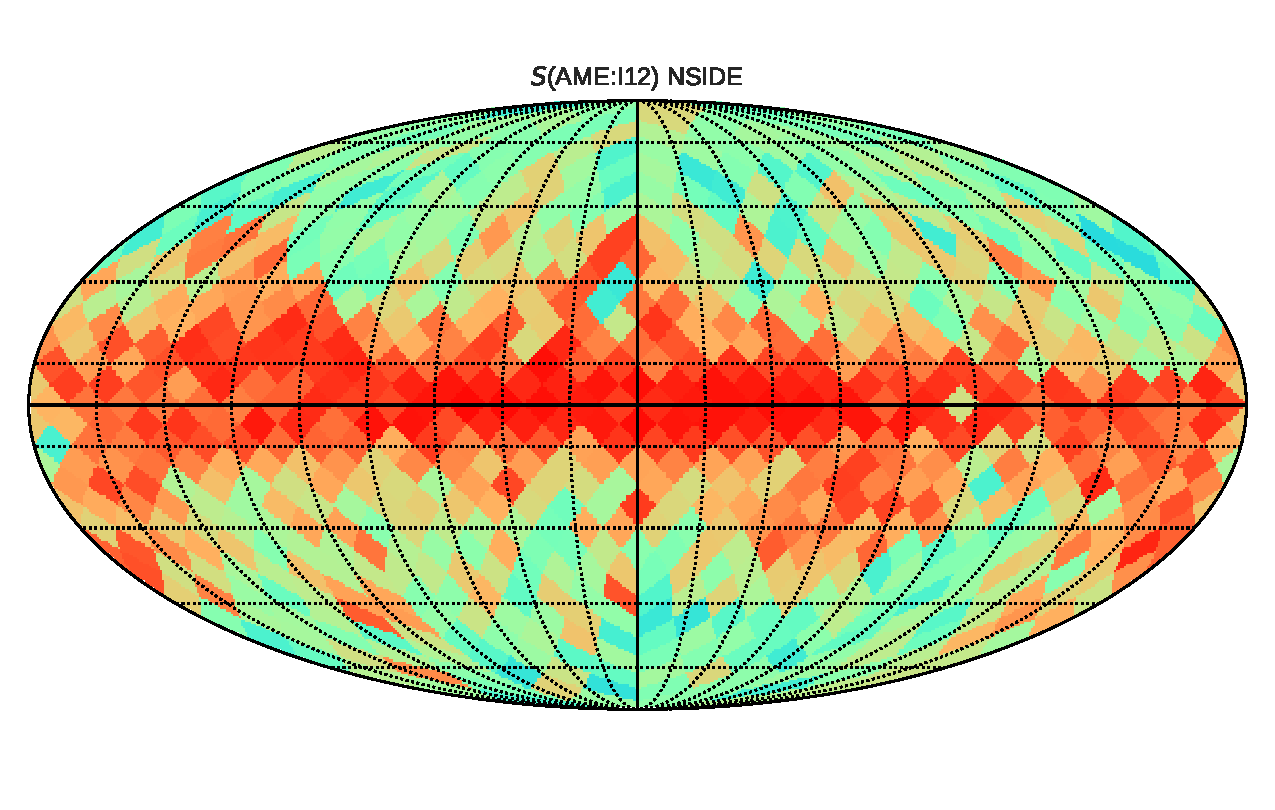
\includegraphics[width=\textwidth]{../Plots/Allsky_Corr/Spearman_Map_nside8_AMEtoI12.pdf}
        \centering
        \caption{}
        \label{fig:Spearman_Map_nside8_AMEtoIR}
      \end{figure}

      \begin{figure}
        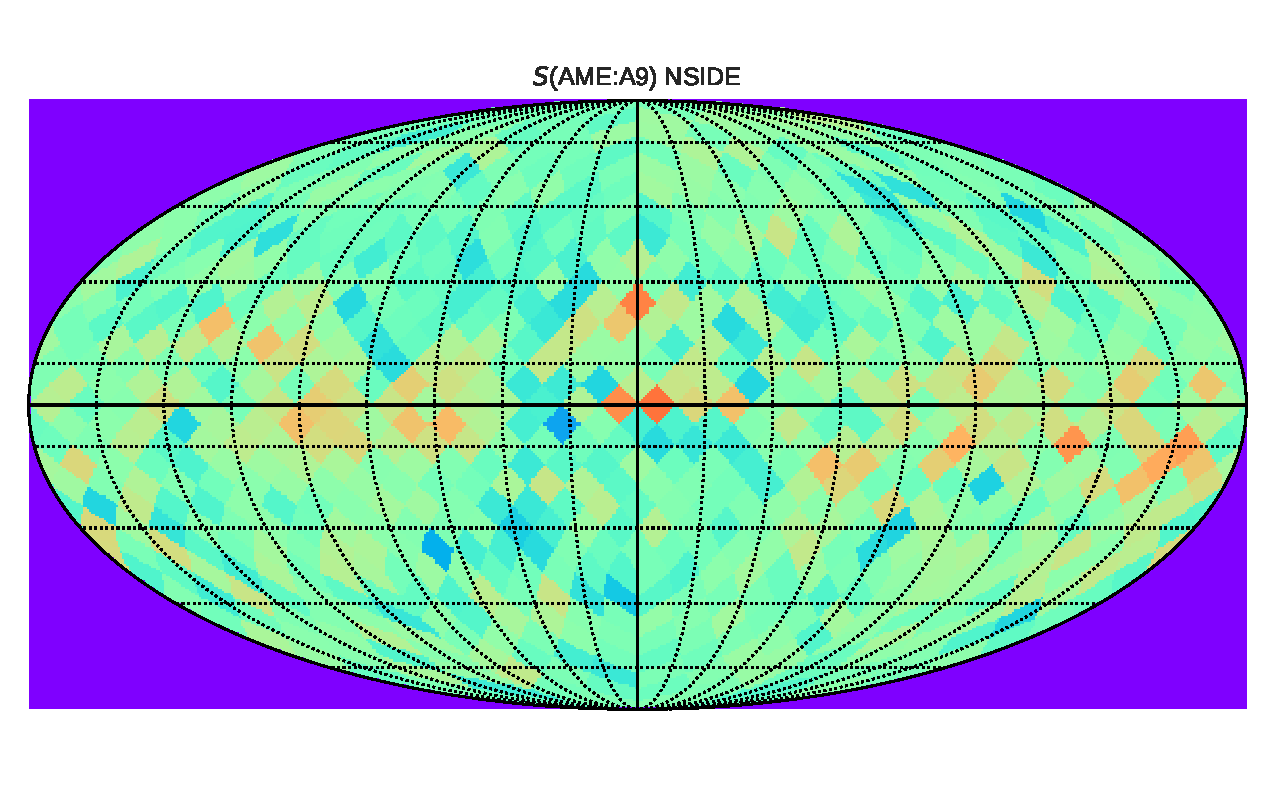
\includegraphics[width=\textwidth/3]{../Plots/Allsky_Corr/RadNorm/Spearman_Map_nside8_AMEtoA9.pdf}
        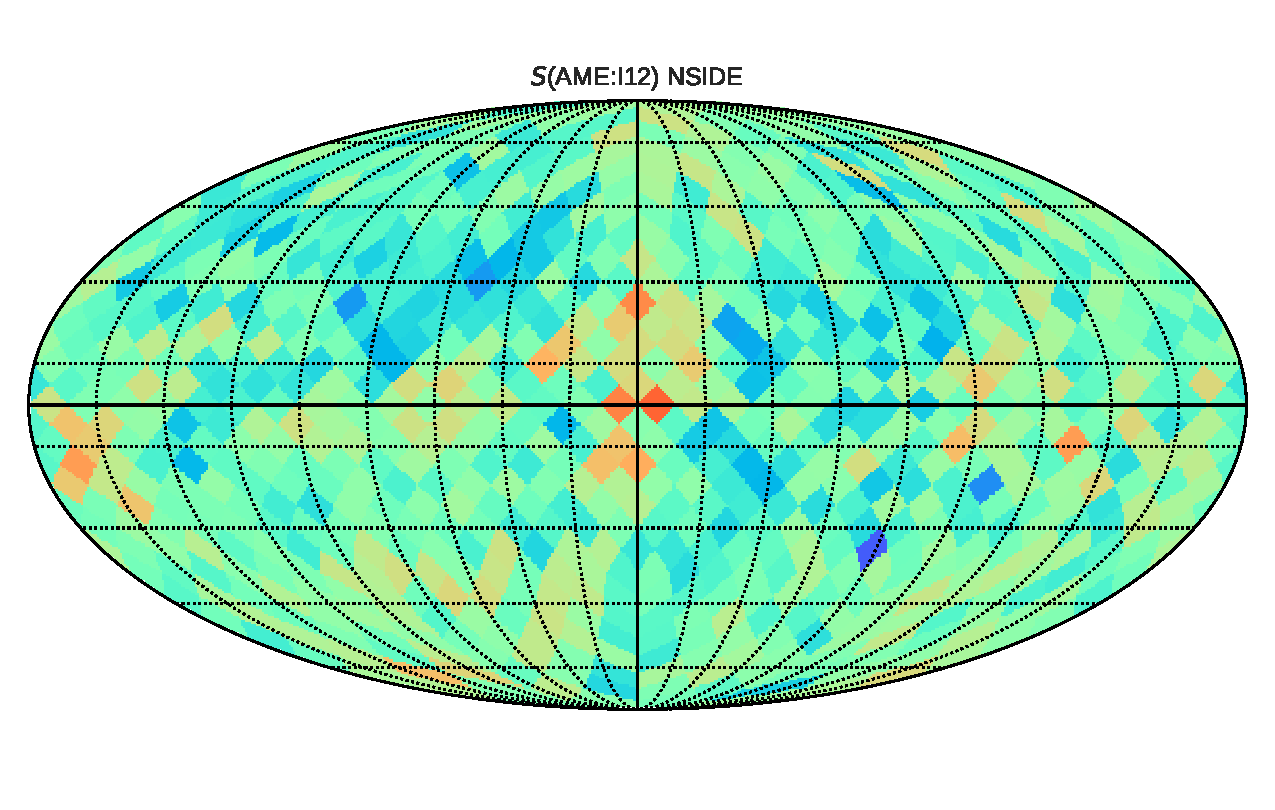
\includegraphics[width=\textwidth/3]{../Plots/Allsky_Corr/RadNorm/Spearman_Map_nside8_AMEtoI12.pdf}
        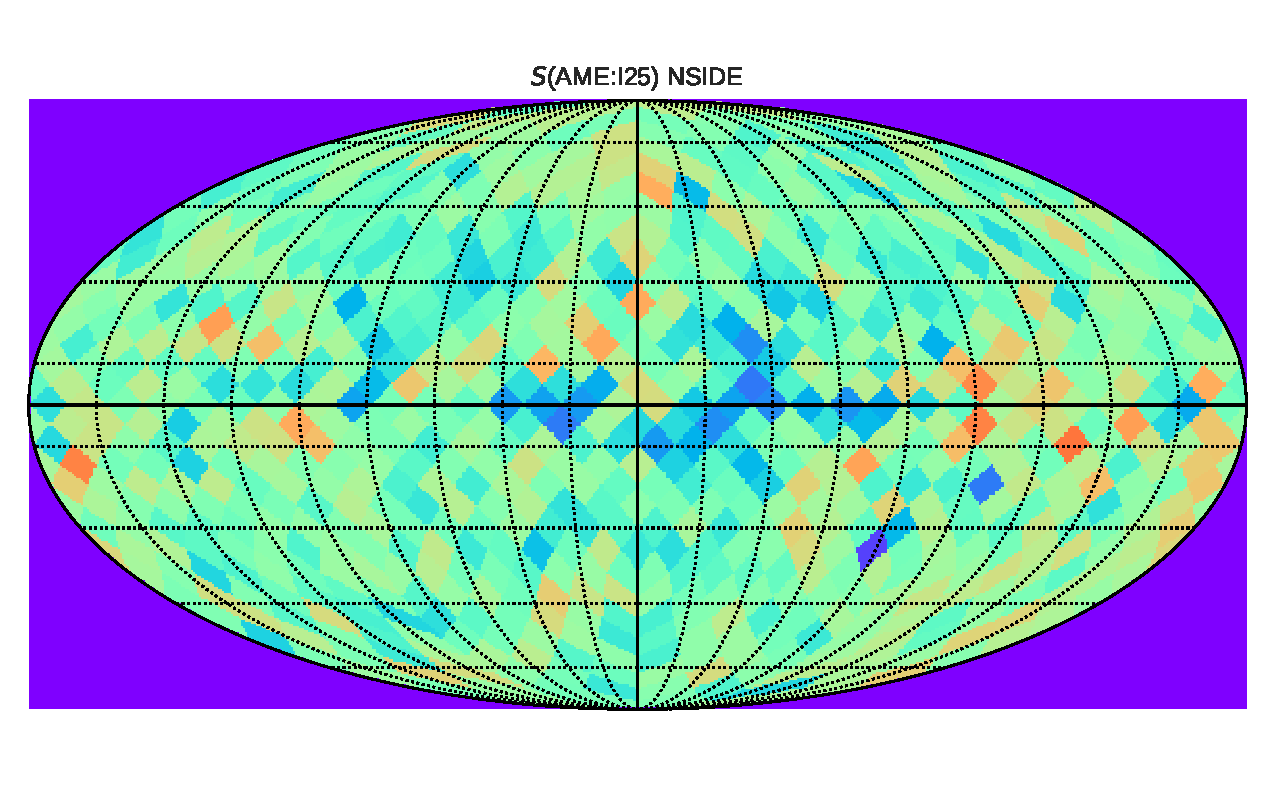
\includegraphics[width=\textwidth/3]{../Plots/Allsky_Corr/RadNorm/Spearman_Map_nside8_AMEtoI25.pdf}
        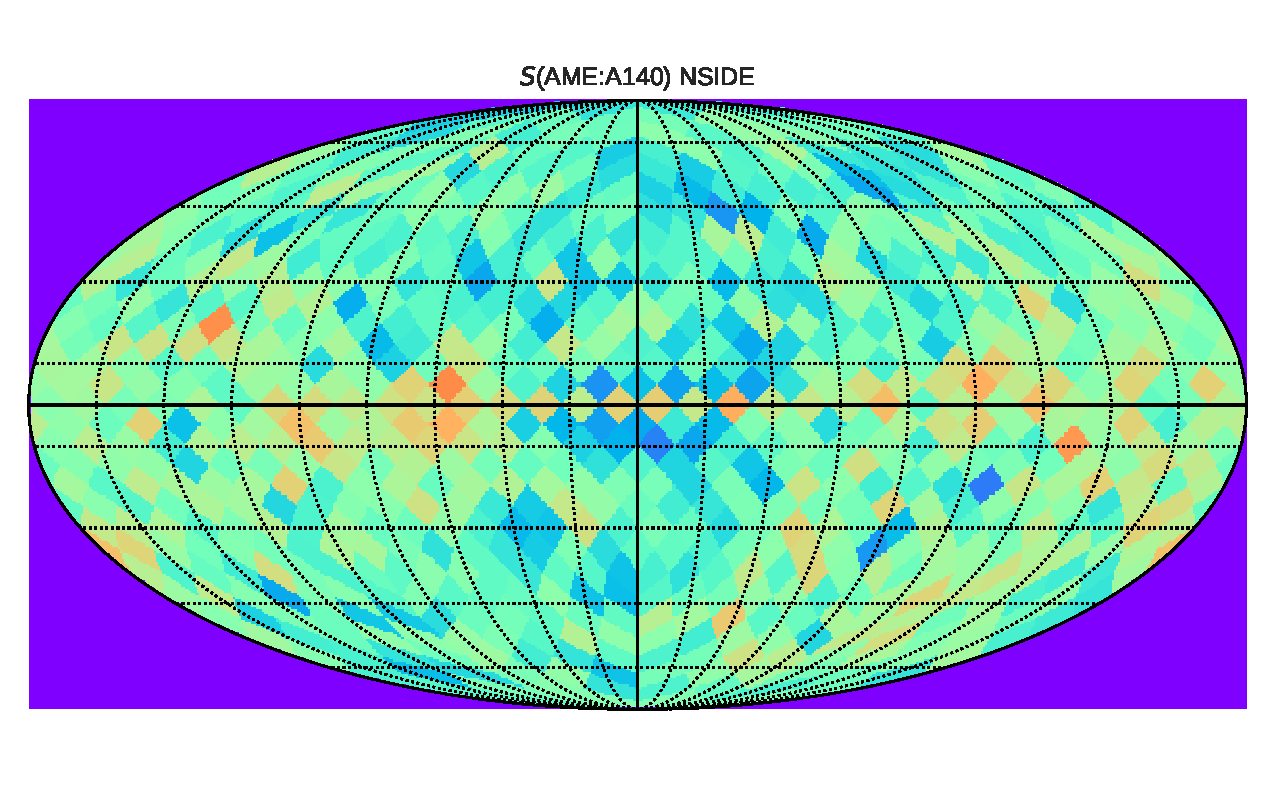
\includegraphics[width=\textwidth/3]{../Plots/Allsky_Corr/RadNorm/Spearman_Map_nside8_AMEtoA140.pdf}
        \centering
        \caption{Spatial map of $r_{s}$ between the AME and IR intensity as in Fig. \ref{fig:Spearman_Map_nside8_AMEtoIR}, but with the AME and IR maps first normalized by dust radiance $R$.}
        \label{fig:Spearman_Map_nside8_AMEtoIR_radnorm}
     \end{figure}

    \section{Discussion}
      \subsection{AME:Dust}
        As noted in Ch. \hyperref[ch:intro]{\ref{ch:intro}}, previous studies found that the AME generally correlates at dust-related IR wavelengths \citep{ysard10b,planckXV, hensley16}. We see the same overall pattern in the present study.

         In our all-sky comparison, we find a first-order correlation between IR intensity and AME intensity, for each of the 12 wavelengths sampled. This is again consistent with the previous investigations of the AME cited above, in that the FIR emission shows the tightest correlation with the AME intensity.

         In testing for a second-order correlation, we divided the IR intensities and AME intensity by the dust radiance, and again performed the band-by-band all-sky comparison. There is evidence of a residual correlation between $I_{MIR}$ and $I_{AME}/R$. Unsurprisingly, the strong correlation between $I_{FIR}$ and $I_{AME}$ disappears when scaling by $R$, as the the FIR bands are dominated by thermal dust emission. In this case, we again find no evidence of an improved correlation for the PAH-dominated bands.

           The closeness of the correlation coefficients found here is consistent with the results of the IRAS vs. AME correlation test result from \cite{planckXV}. They found that the correlation coefficient among the 4 IRAS bands (12, 25, 60, and 100~$\mu$m) differ from one another only by about 5\%, across the whole set of 98 regions. The trend of AKARI MIR and FIR data vs. the AME does not disagree with their IRAS comparison. This work adds that bands longer than IRAS 100~$\mu$m also correlate strongly with AME, especially the two Planck/HFI bands used.

          \subsection{AME:PAH}
            Each of the bands sampled show correlation with the AME, however the FIR bands always show the strongest correlation. In fact, the correlation pattern of AME vs. each of the IR bands, very strongly resembles the correlation results of the Planck HFI bands vs. all of the other bands (Fig. \ref{fig:AME_IR_crosscorr_allbandsg}.) This is readily apparent from the pixel-density plots in Fig. \ref{fig:AMEvsDust_allsky_allbands}, wherein the FIR bands pixels show a very similar density profile vs. the AME. In attempting to factor out this first-order correlation, dividing the AME and IR intensities by the dust radiance for each pixel, we find the there is still a residual correlation between the MIR bands and the AME. The FIR bands scaled by the dust radiance, as expected, lack correlation with $I_{AME}/R$.

          \subsection{AME:$T$, $G_{0}$}
            According to spinning dust theory outlined in \cite{draine98a} and in subsequent works by \cite{ysard10a}, the AME profile and intensity will depend in part on the ISRF- but as is well-stated in \cite{hensley17a}, exactly how the ISRF will affect the AME SED is a more complicated question. Absorbed starlight photons may be able to rotationally excite the carriers, but if an enhanced ISRF leads to increased dust heating, then the increased IR emission can rotationally de-excite the carriers. However the ISRF affects not only the dust temperature but ionization of the carriers.

            \cite{hensley16} looked at the $AME$/$R$ ratio vs. $T$ and found only a slight anti-correlation of $P = -0.06$.

          \subsection{Microwave foreground component separation}

            There are known degeneracies between the foreground parameters of the COMMANDER maps (spinning-dust, and free-free, synchrotron components as described in \cite{planck15X}.) This can be demonstrated by comparing the ratio map of the PCXV intensity to thermal dust intensity.
